%%%%%%%%%%%%%%%%%%%%%%%%%%%%%%%%%%%%%%%%%
% Short Sectioned Assignment
% LaTeX Template
% Version 1.0 (5/5/12)
%
% This template has been downloaded from: http://www.LaTeXTemplates.com
% Original author: % Frits Wenneker (http://www.howtotex.com)
% License: CC BY-NC-SA 3.0 (http://creativecommons.org/licenses/by-nc-sa/3.0/)
% Modified by Alan G. Labouseur  - alan@labouseur.com, and Ryan Munger - ryan.munger1@marist.edu
%
%%%%%%%%%%%%%%%%%%%%%%%%%%%%%%%%%%%%%%%%%

%----------------------------------------------------------------------------------------
%	PACKAGES AND OTHER DOCUMENT CONFIGURATIONS
%----------------------------------------------------------------------------------------

\documentclass[letterpaper, 10pt]{article} 

\usepackage{tikz}
\usetikzlibrary{automata, positioning}
\usepackage[english]{babel} % English language/hyphenation
\usepackage{graphicx}
\usepackage[lined,linesnumbered,commentsnumbered]{algorithm2e}
\usepackage{listings}
\usepackage{float}
\usepackage{fancyhdr} % Custom headers and footers
\pagestyle{fancyplain} % Makes all pages in the document conform to the custom headers and footers
\usepackage{lastpage}
\usepackage{url}
\usepackage{xcolor}
\usepackage{titlesec}
\usepackage{ulem}

% Stolen from https://www.overleaf.com/learn/latex/Code_listing 
\definecolor{codegreen}{rgb}{0,0.6,0}
\definecolor{codegray}{rgb}{0.5,0.5,0.5}
\definecolor{codepurple}{rgb}{0.58,0,0.82}
\definecolor{backcolour}{rgb}{0.95,0.95,0.92}

\lstdefinestyle{mystyle}{
    backgroundcolor=\color{backcolour},   
    commentstyle=\color{codegreen},
    keywordstyle=\color{magenta},
    numberstyle=\tiny\color{codegray},
    stringstyle=\color{codepurple},
    basicstyle=\ttfamily\footnotesize,
    breakatwhitespace=false,         
    breaklines=true,                 
    captionpos=b,                    
    keepspaces=true,                 
    numbers=left,                    
    numbersep=5pt,                  
    showspaces=false,                
    showstringspaces=false,
    showtabs=false,                  
    tabsize=2
}
\lstset{style=mystyle, language=c++}


\fancyhead{} % No page header - if you want one, create it in the same way as the footers below
\fancyfoot[L]{} % Empty left footer
\fancyfoot[C]{page \thepage\ of \pageref{LastPage}} % Page numbering for center footer
\fancyfoot[R]{}

\renewcommand{\headrulewidth}{0pt} % Remove header underlines
\renewcommand{\footrulewidth}{0pt} % Remove footer underlines
\setlength{\headheight}{13.6pt} % Customize the height of the header

%----------------------------------------------------------------------------------------
%	TITLE SECTION
%----------------------------------------------------------------------------------------

\newcommand{\horrule}[1]{\rule{\linewidth}{#1}} % Create horizontal rule command with 1 argument of height

\title{	
   \normalfont \normalsize 
   \textsc{CMPT 432 - Spring 2025 - Dr. Labouseur} \\[10pt] % Header stuff.
   \horrule{0.5pt} \\[0.25cm] 	% Top horizontal rule
   \huge Lab 7 -- Semantic Analysis \\     	    % Assignment title
   \horrule{0.5pt} \\[0.25cm] 	% Bottom horizontal rule
}

\author{Ryan Munger \\ \normalsize Ryan.Munger1@marist.edu}

\date{\normalsize\today} 	% Today's date.

\begin{document}

\maketitle % Print the title

%----------------------------------------------------------------------------------------
%   CONTENT SECTION
%----------------------------------------------------------------------------------------

% - -- -  - -- -  - -- -  -
\vspace{-.7cm}

\subsection{Scope and Type Checking}
Explain in detail what is happening in the diagram below.

\begin{figure} [h]
    \centering
    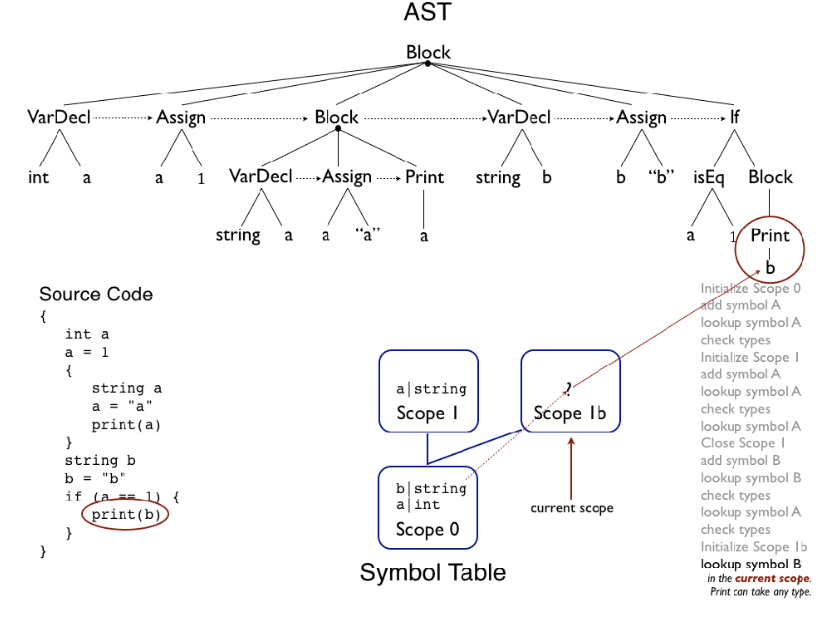
\includegraphics[width=1\linewidth]{diagram.png}
    \caption{AST Diagram}
    \label{fig:enter-label}
\end{figure}
\newpage

The diagram depicts an Abstract Syntax Tree (AST) and some evaluations of it. As we can see, we examined the source code to produce the Symbol Table and build the tree. We start with an open block. This is the root of our tree and initializes Symbol Table 0. As we go through the code, we detect statements and add them accordingly. For example, the first thing we see after the open block is \textit{int a}. We then add a \textit{VarDecl} to our AST and the symbol \textit{a} as type \textit{int} in our current symbol table (after ensuring \textit{a} is not already in use!). This process continues very similarly to our parser. When \textit{a = 1} is reached, we add an \textit{Assign} to our AST. Since we are not declaring a new symbol, we must verify that we are using the existing entry correctly. We look up \textit{a} and find that it is of type \textit{int}. Since we are assigning a value of the correct type to \textit{a}, we may continue. Skipping ahead, we can see that \textit{Print b} is of special interest in this diagram. Since \textit{if} statements have their own symbol table (they possess scope), we are in scope 1b. We now look up the symbol \textit{b}, which is to be printed, in the most local scope. Since \textit{b} is not declared in scope 1b, we must move up. Scope 1b's parent scope, scope 0, is checked next. Scope 0 has symbol \textit{b} defined as a string. Since \textit{print} may take any type and symbol \textit{b} is defined, we are good to go! Happy semantic analysis!
\end{document}